% ML4QS Practical Report - Intermediate Deadline 2 (max 5 pages excl. references)
% LLNCS format, Springer Lecture Notes in Computer Science
%
\documentclass[runningheads]{llncs}

\usepackage{graphicx}
\graphicspath{{figures/}{./}}
\usepackage{booktabs}
\usepackage{amsmath}
\usepackage{hyperref}
\usepackage{xcolor}
\usepackage{microtype}

\renewcommand\UrlFont{\color{blue}\rmfamily}

\begin{document}

\title{Recognizing Everyday Hand Activities from Wrist Sensor Data for Digital Wellbeing Applications}

\titlerunning{Recognizing Hand Activities from Wrist Sensor Data}

\author{Aniket Dasurkar \and Mansi Saxena \and Shreya Bhatt}
\authorrunning{A. Dasurkar et al.}
\institute{Vrije Universiteit Amsterdam, Amsterdam, The Netherlands}

\maketitle

\begin{abstract}
We study whether a wrist-worn smartphone can tell apart five everyday hand activities: smoking, typing, idle, cooking, and dumbbell exercising. From the raw inertial signals collected earlier in this project we build a set of time-domain, frequency-domain, and axis-correlation features over short windows, then train and compare several classical classifiers. The hard part is generalising to a new person, so we train on two subjects and test on a third who recorded independently. A stacking ensemble of an SVM, a random forest, a kNN, and a decision tree reaches about 93\% accuracy on this unseen subject, ahead of voting ensembles and every single model. We also report an honest gap: grouped cross-validation predicts new-recording performance well, but a leave-one-subject-out check shows that a genuinely new person is far harder. These results set the baseline that motivates the deep-learning stage.

\keywords{Activity recognition \and Feature engineering \and Classical machine learning \and Ensemble learning \and Wrist sensors}
\end{abstract}


% ─────────────────────────────────────────────────────────────
\section{Introduction}
\label{sec:intro}
% ─────────────────────────────────────────────────────────────

A smartphone on the wrist records how the hand moves all day. If we can turn that motion into a label for what the person is doing, we have the building block for a digital wellbeing assistant. Such an assistant could track how often someone smokes, how long they sit typing, how much time goes into cooking, and how much into exercise, with no manual logging. That is the practical problem behind this project.

In the earlier stage we strapped a phone to the dominant wrist with a sports armband and recorded accelerometer, gyroscope, and linear accelerometer data through Phyphox~\cite{phyphox2019}. Three subjects each performed the five activities in several short sessions. We train on two of them (subject\_1 and subject\_3) and keep the third (subject\_2) fully held out for testing. Subject\_2 recorded independently, so test accuracy reflects how the system would work for a new user, not a familiar one.

This report covers feature engineering and classical modelling. The question we answer is concrete: \emph{given short windows of wrist motion, can a classical classifier built on engineered time- and frequency-domain features recognise these five activities, and how well does it transfer to a person it has never seen?} Section~\ref{sec:features} describes the features and analyses which ones actually help. Section~\ref{sec:models} defines the train/test setup, the model line-up, and how we tuned each model. Section~\ref{sec:discussion} presents the results and discusses where they hold up and where they do not. Section~\ref{sec:conclusion} concludes.


% ─────────────────────────────────────────────────────────────
\section{Feature Engineering}
\label{sec:features}
% ─────────────────────────────────────────────────────────────

Classical models need a fixed-length vector per example, so we summarise each short slice of signal into features following Chapter~4 of the course book~\cite{hoogendoorn2018}. All signals are resampled to \textbf{50\,Hz}. The earlier exploratory analysis showed that almost all relevant motion sits below about 12\,Hz, so 50\,Hz leaves comfortable headroom and matches typical consumer wearables.

\subsection{Window size}
We slice the signal into \textbf{2-second windows with 50\% overlap} (a 1-second step). The first report had promised 4-second windows, and we changed that on purpose. Two seconds still captures the dominant rhythm of every activity we care about, it produces roughly twice as many windows (more training examples), and shorter windows mix fewer distinct sub-movements together. We do not claim 2\,s captures a full smoking cycle, which is slower than that. It captures enough of the repeating motion to be informative, and the extra examples were worth more to us than fitting one whole cycle per window. After windowing the data set is \textbf{3{,}360 windows}, balanced across activities (672 each), split into \textbf{2{,}240 training} windows (subject\_1 + subject\_3) and \textbf{1{,}120 test} windows (subject\_2).

\subsection{The three feature families}
For every window we compute three groups of features, applied to all twelve signals: the nine raw axes of the three sensors plus three magnitude channels that fold each sensor's axes into one. The groups are summarised in Table~\ref{tab:features}.

\begin{itemize}
  \item \textbf{Time-domain (156 features).} How much the wrist moves and what shape that motion has. Mean, standard deviation, range, RMS, signal magnitude area, peak-to-peak, IQR, MAD, zero-crossing rate, skewness, and kurtosis. These separate a smooth swing from a burst of sharp taps.
  \item \textbf{Frequency-domain (84 features).} The rhythm of the motion, from an FFT of each window. Dominant frequency, spectral energy, and spectral entropy. These pick up the speed differences seen in the earlier analysis.
  \item \textbf{Axis-correlation (9 features).} Whether the three directions move together, via pairwise correlations (x--y, x--z, y--z) on each sensor. A coordinated arm swing and a one-directional tap differ here.
\end{itemize}

\begin{table}[ht]
\caption{Feature groups computed for every 2-second window (50\,Hz, 50\% overlap).}
\label{tab:features}
\centering\small
\setlength{\tabcolsep}{4pt}
\begin{tabular}{p{2.1cm}cp{4.2cm}p{3.1cm}}
\toprule
\textbf{Group} & \textbf{Count} & \textbf{What it captures} & \textbf{Examples} \\
\midrule
Time domain      & 156 & strength, variability and shape of motion & RMS, SMA, range, MAD, skewness \\
Frequency domain & 84  & speed and regularity of motion & dominant freq., spectral energy, spectral entropy \\
Axis correlation & 9   & whether the three axes move together & corr.\ x--y, x--z, y--z \\
\midrule
\textbf{Total} & \textbf{249} & & \\
\bottomrule
\end{tabular}
\end{table}

A few windows produced undefined values, for example skewness on a near-constant idle window. We imputed these with the median of each feature computed on the \emph{training} windows only, so nothing about the test subject leaked into preprocessing. That leaves a clean $3{,}360 \times 249$ table.

\subsection{Is the feature set actually useful?}
To check whether each family earns its place, we trained a random forest on each group alone and on the full set, using the same person-independent split. The results are in Table~\ref{tab:ablation}.

\begin{table}[ht]
\caption{Feature-group ablation (random forest, held-out subject\_2).}
\label{tab:ablation}
\centering\small
\begin{tabular}{lccc}
\toprule
\textbf{Feature set} & \textbf{\# features} & \textbf{Test accuracy} & \textbf{Test macro-F1} \\
\midrule
Time-domain only      & 156 & 0.8955 & 0.8926 \\
Frequency-domain only & 84  & 0.8268 & 0.8236 \\
Correlation only      & 9   & 0.4732 & 0.4601 \\
All features          & 249 & 0.8884 & 0.8858 \\
\bottomrule
\end{tabular}
\end{table}

The time-domain block carries most of the signal: alone it reaches 0.8955 accuracy. Frequency features alone manage 0.8268, useful but clearly secondary. The nine correlation features alone reach only 0.4732, well above the 0.20 random baseline but far too weak to stand on their own. One result surprised us. The full set (0.8884) scored slightly \emph{below} time-domain alone (0.8955). The most likely reason is redundancy and noise: with 191 feature pairs at $|r| > 0.95$, the extra columns mostly repeat information already present, and a few weak frequency and correlation features dilute the forest's splits. We kept all 249 features anyway, because the strong models we actually deploy (SVM with standardisation, ensembles) handle redundant inputs well, and because hand-pruning would add a design choice with little payoff at this dataset size.

The random-forest importances tell the same story (Fig.~\ref{fig:importance}). The top features are \texttt{acc\_y\_rms} (0.0343) and \texttt{acc\_y\_sma} (0.0340), both plain measures of how much the vertical accelerometer axis moves. Gyroscope spread features follow: \texttt{gyr\_mag\_p2p}, \texttt{gyr\_x\_rms}, \texttt{gyr\_mag\_range}, \texttt{gyr\_x\_mad}. The first frequency feature, \texttt{gyr\_x\_spec\_energy}, appears only at rank 9 (0.0143). So for tree-based models the amount and variability of wrist motion dominate, and rhythm adds a smaller increment. That matches the ablation.

\begin{figure}[ht]
  \centering
  
\includegraphics[width=0.72\textwidth]{figures/rf_feature_importance.png}
  \caption{Top-20 random-forest feature importances (trained on subject\_1 + subject\_3, all 249 features). Time-domain spread features of the accelerometer and gyroscope dominate; the first frequency feature appears only at rank 9.}
  \label{fig:importance}
\end{figure}


% ─────────────────────────────────────────────────────────────
\section{Train/Test Setup and Models}
\label{sec:models}
% ─────────────────────────────────────────────────────────────

\subsection{Person-independent split}
We train on subject\_1 and subject\_3 (2{,}240 windows) and test on the held-out subject\_2 (1{,}120 windows), each set balanced across the five activities. Subject\_2 never appears in training or model selection. All 249 features are standardised to zero mean and unit variance using training statistics only, then applied unchanged to the test windows. The whole pipeline is built with scikit-learn~\cite{pedregosa2011}.

\subsection{Model line-up}
We compared classical models with different inductive biases, then stacked and voted over the strongest ones (course book Ch.~7~\cite{hoogendoorn2018}).
\begin{itemize}
  \item \textbf{kNN} and \textbf{Naive Bayes}: light-assumption baselines.
  \item \textbf{Decision Tree}: one interpretable model.
  \item \textbf{Random Forest}: many trees, robust, gives feature importances.
  \item \textbf{SVM (RBF)}: curved boundaries for subtle cases like smoking vs.\ idle.
  \item \textbf{Gradient Boosting}: sequential trees that fix earlier errors.
  \item \textbf{Voting (hard / soft)} and \textbf{Stacking}: combine the tuned base learners.
\end{itemize}

The reason to ensemble is simple. The base learners make different kinds of mistakes, so combining them cancels some error. Hard voting takes the majority label, soft voting averages class probabilities. Stacking goes one step further: a logistic-regression meta-learner is trained on the base models' outputs and learns which base model to trust for which case. That is why stacking edges out plain voting here.

\subsection{Hyperparameter optimization}
Every tunable model was tuned with \texttt{GridSearchCV} under \textbf{GroupKFold}, grouped by recording session (see Sect.~\ref{sec:cv}). The grids and chosen settings are in Table~\ref{tab:grids}. Naive Bayes was left at defaults. The ensembles reuse these tuned base learners directly.

\begin{table}[ht]
\caption{Grids searched (GridSearchCV under GroupKFold) and selected settings.}
\label{tab:grids}
\centering\small
\setlength{\tabcolsep}{4pt}
\begin{tabular}{lp{5.8cm}p{2.2cm}}
\toprule
\textbf{Model} & \textbf{Grid searched} & \textbf{Selected} \\
\midrule
kNN & \texttt{n\_neighbors} $\in \{1,3,5,7,9,11,15\}$ & $k=3$ \\
Decision Tree & \texttt{max\_depth} $\in \{3,5,7,10,15,\text{None}\}$ & depth $=7$ \\
Random Forest & \texttt{n\_estimators}$\in\{100,200,300\}$, \texttt{max\_depth}$\in\{$None$,10,20\}$, \texttt{max\_features}$\in\{$sqrt$,0.3\}$ & 300, None, 0.3 \\
SVM (RBF) & \texttt{C}$\in\{0.1,1,10,100\}$, \texttt{gamma}$\in\{$scale$,0.001,0.01,0.1\}$ & $C{=}100$, $\gamma{=}0.001$ \\
Gradient Boosting & \texttt{n\_estimators}$\in\{100,200\}$, \texttt{learning\_rate}$\in\{0.05,0.1\}$, \texttt{max\_depth}$\in\{2,3\}$ & lr 0.1, depth 2, 200 \\
Naive Bayes & none (GaussianNB defaults) & defaults \\
\bottomrule
\end{tabular}
\end{table}

\subsection{Why GroupKFold, not shuffled K-fold}
\label{sec:cv}
Our windows overlap by 50\%, so two consecutive windows from the same recording share half their samples. A plain shuffled K-fold would scatter such near-duplicate windows across train and validation folds. The model could then memorise a recording rather than learn the activity, and the CV score would be inflated. We saw exactly this in an earlier run: shuffled CV made kNN with $k=1$ look like the winner, which is the classic sign of leakage through near-duplicate neighbours.

GroupKFold fixes this by grouping all windows from one recording into the same fold, so overlapping windows never split across folds. Every CV number we report comes from this leakage-free setup. It is a deliberate methodological choice and it changed which models we trusted.


% ─────────────────────────────────────────────────────────────
\section{Results and Discussion}
\label{sec:discussion}
% ─────────────────────────────────────────────────────────────

Table~\ref{tab:results} lists every model with its grouped-CV accuracy and its held-out test accuracy and macro-F1 (the selected hyperparameters are in Table~\ref{tab:grids}). Figure~\ref{fig:comparison} plots the four test metrics with the random baseline.

\begin{table}[ht]
\caption{All models, sorted by test macro-F1. Grouped-CV is on the training subjects; test is the held-out subject\_2. Selected hyperparameters are given in Table~\ref{tab:grids}.}
\label{tab:results}
\centering\small
\begin{tabular}{lccc}
\toprule
\textbf{Model} & \textbf{CV acc} & \textbf{Test acc} & \textbf{Test F1} \\
\midrule
\textbf{Stacking (SVM+RF+kNN+DT $\to$ LR)} & 0.9920 & \textbf{0.9295} & \textbf{0.9287} \\
Voting (hard) & 0.9924 & 0.9277 & 0.9271 \\
Voting (soft) & 0.9929 & 0.9223 & 0.9213 \\
Gradient Boosting & 0.9893 & 0.9036 & 0.9016 \\
SVM (RBF) & 0.9915 & 0.8893 & 0.8892 \\
kNN & 0.9920 & 0.8848 & 0.8840 \\
Naive Bayes & 0.9353 & 0.8812 & 0.8792 \\
Random Forest & 0.9879 & 0.8804 & 0.8762 \\
Decision Tree & 0.9362 & 0.8250 & 0.8197 \\
\bottomrule
\end{tabular}
\end{table}

\begin{figure}[ht]
  \centering
  
\includegraphics[width=0.88\textwidth]{figures/model_comparison.png}
  \caption{Accuracy, macro-F1, precision, and recall on the held-out subject\_2 for all models (standardised features). The dashed line marks the 0.20 accuracy of random guessing among five classes. The ensembles lead, with stacking on top.}
  \label{fig:comparison}
\end{figure}

\subsection{Stacking is the best model}
The headline result is the stacking ensemble: \textbf{0.9295 test accuracy and 0.9287 macro-F1} on the unseen subject. It beats hard voting (0.9277) and soft voting (0.9223), and sits well clear of the best single models, gradient boosting (0.9036) and SVM (0.8893). The single tree-based and distance-based models cluster near 0.88, and the lone decision tree trails at 0.825. The pattern is exactly what we hoped for when we built the ensembles: the base learners disagree on different windows, and the meta-learner exploits that disagreement. The lift from the best single model (SVM, 0.8893) to stacking (0.9295) is about four points, which is real and consistent across all four metrics in Fig.~\ref{fig:comparison}.

\subsection{Where the mistakes are}
Figure~\ref{fig:confusion} is the normalised confusion matrix for the stacking model. Per-class F1 ranges from 0.991 (idle) and 0.969 (typing) down to 0.878 (smoking) and 0.879 (cooking). Idle and typing are nearly clean, which fits intuition: idle barely moves and typing has a distinctive fast low-amplitude pattern. The errors concentrate where we expected from the EDA. Cooking is the messiest activity and leaks into both smoking (19 windows) and exercising (18), because it mixes slow arm motions that look like smoking with fast ones that look like exercise. Smoking spreads the other way, into cooking (10), exercising (10), and typing (8). These three (smoking, cooking, idle/typing at the low-motion end) were always the ambiguous cases, and the confusion matrix confirms it rather than surprising us.

\begin{figure}[ht]
  \centering
  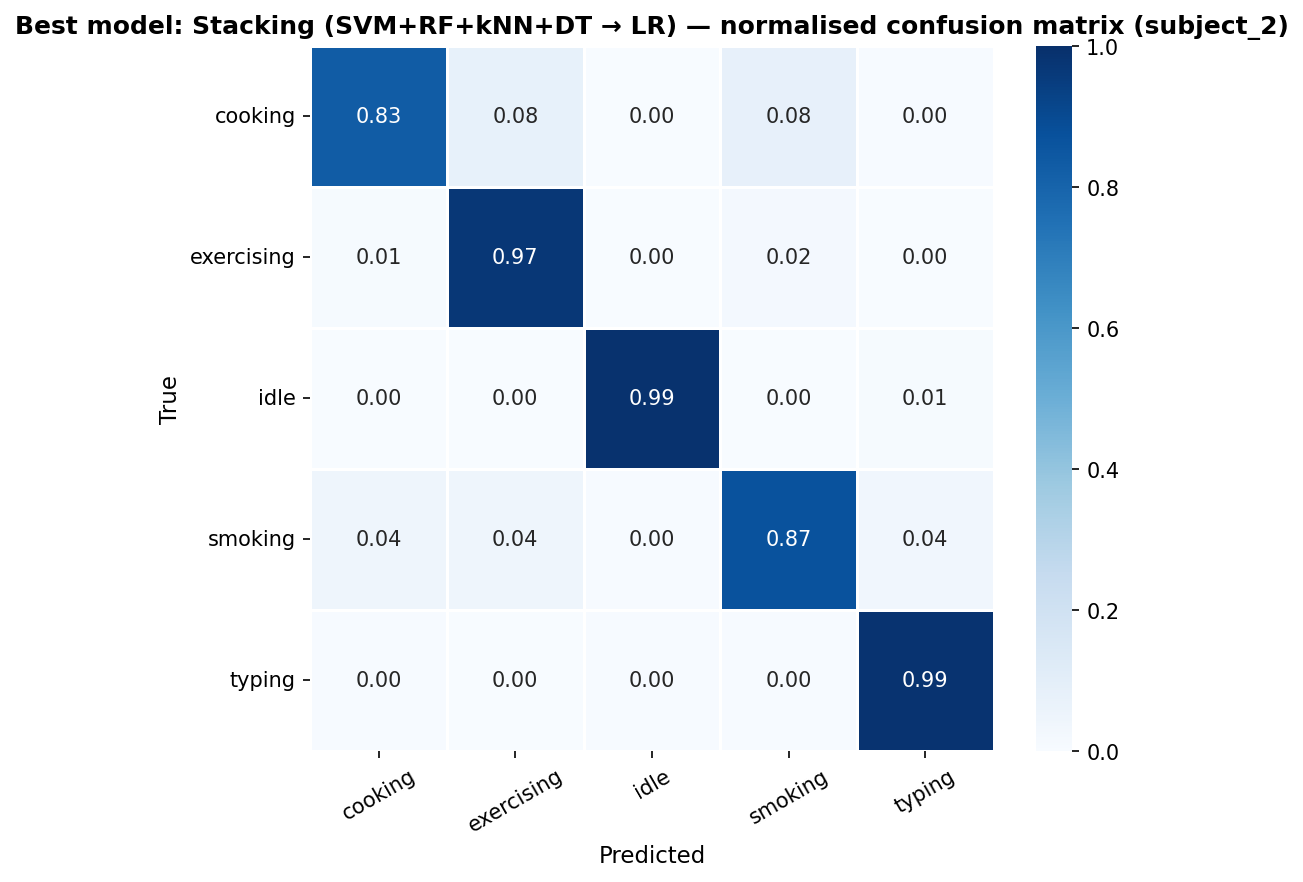
\includegraphics[width=0.52\textwidth]{figures/cm_best.png}
  \caption{Normalised confusion matrix of the stacking model on the held-out subject\_2 (standardised features). Rows are true activities. Cooking and smoking are the main sources of error; idle and typing are nearly clean.}
  \label{fig:confusion}
\end{figure}

\subsection{Grouped-CV vs.\ a genuinely new person: an honest gap}
\label{sec:honesty}
Grouped-CV reports about 0.99 for the top models, while held-out test sits near 0.93. For stacking the gap is only $+0.0625$ (0.9920 vs.\ 0.9295), and for the other ensembles it is similar. So grouped-CV is an honest predictor of performance on a \emph{new recording from a known person}. That is a useful guarantee, but it is not the hardest case.

The hardest case is a genuinely new person. To probe that, we ran leave-one-subject-out (train on one training subject, validate on the other). The numbers drop sharply: stacking 0.5455, SVM 0.5286, random forest 0.4879. With only three subjects this is a small, noisy estimate, but the message is clear and we are not hiding it. Recognising activities for a person in the training distribution is close to solved here. Recognising activities for a truly new individual, whose personal motion style we have never observed, is much harder, and two training subjects are simply not enough to cover that variation. This is the main limitation of the current setup.

\subsection{Answering the research question}
Yes, a classical classifier on engineered time- and frequency-domain features recognises these five activities well for the held-out subject, reaching 0.9295 accuracy and 0.9287 macro-F1, far above the 0.20 random baseline. The win comes from ensembling complementary base learners rather than from any single clever model. The honest caveat is that this holds for a subject drawn from the same small pool; the LOSO result shows the jump to a brand-new person is still open.


% ─────────────────────────────────────────────────────────────
\section{Conclusion}
\label{sec:conclusion}
% ─────────────────────────────────────────────────────────────

From one hour of wrist motion we engineered 249 features per 2-second window and compared nine classical setups under a strict person-independent split. Time-domain spread features did most of the work; frequency features helped less and correlation features barely at all on their own. A stacking ensemble of a tuned SVM, random forest, kNN, and decision tree was the best model, at 0.9295 accuracy and 0.9287 macro-F1 on the held-out subject. The remaining errors sit around cooking and smoking, the two least repeatable activities, and the leave-one-subject-out check shows that generalising to a completely new person remains the real challenge. That gap, plus the fact that our features are hand-designed window statistics, is what motivates the deep-learning stage: a model that learns representations directly from the raw time series may close some of the distance to a genuinely new user.


% ─────────────────────────────────────────────────────────────
\begin{thebibliography}{9}

\bibitem{hoogendoorn2018}
Hoogendoorn, M., Funk, B.: Machine Learning for the Quantified Self. Springer (2018)

\bibitem{pedregosa2011}
Pedregosa, F., Varoquaux, G., Gramfort, A., et al.: Scikit-learn: Machine learning in Python.
Journal of Machine Learning Research \textbf{12}, 2825--2830 (2011)

\bibitem{rabbi2015mybehavior}
Rabbi, M., Aung, M.H., Zhang, M., Choudhury, T.: MyBehavior: Automatic personalized health feedback from user behaviors and preferences using smartphones.
In: Proceedings of the ACM International Joint Conference on Pervasive and Ubiquitous Computing (UbiComp), pp.~707--718. ACM (2015)

\bibitem{phyphox2019}
Staacks, S., Hutz, S., Heinke, H., Stampfer, C.: Advanced tools for smartphone-based experiments: Phyphox.
Physics Education \textbf{53}(4), 045009 (2018)

\end{thebibliography}

\end{document}
